\chapter{Introduction}
\label{chap:introduction}


\chapter{Log file analysis}
\label{chap:log-analysis}
\todo{Placeholder: ~\cite{he2016expreport, zhu2023loghub}}.

\section{Introduction to log file analysis}
\label{sec:intro-analysis}
Log file analysis~\cite{hulshof2005logfile} is a basic method that offers a significant understanding of cognitive procedures and interaction with computer applications. This process includes the collection, examination, and explanation of information from log files. By employing these techniques, we can understand the behavior of the system, pinpoint problems, and spot irregularities. This chapter is designed to outline the objectives of log file analysis and the techniques that can be employed in the process.

\section{Purpose of log file analysis}
\label{sec:purpose}
The principal aim of analyzing log files~\cite{aivalis2020logfile} is to ensure effective monitoring and management of the system by reviewing log data. This investigative process helps IT administrators and teams effectively oversee and control their systems. Through the examination of log files, they are able to discern patterns, spot irregularities, resolve problems, guarantee system dependability, improve security measures, and boost system efficiency. The application of log file analysis provides an understanding of how these elements affect behavior. Monitoring user behavior is relevant in two scenarios, both practical and scientific.

In a practical context~\cite{hulshof2005logfile}, understanding the approach individuals take when interacting with a computer program can be highly beneficial. As computer usage becomes increasingly prevalent in daily life, human-computer interaction is gaining importance in various domains. With more people interacting with computer applications, there is a growing need to study user behavior and preferences. Analyzing user preferences and typical usage sequences can inform interface design modifications to align with user expectations.

In a scientific context~\cite{hulshof2005logfile}, the way individuals interact with a computer application is of substantial relevance to social science. Numerous studies in education have explored the effectiveness of computer-assisted learning. Although computers can augment the process of learning, many students face difficulties in comprehending the software utilized. A considerable amount of research has been dedicated to understanding how these elements impact learning results, particularly in the context of discovery learning via computer simulations.

\section{Steps and methods of log file analysis}
\label{sec:steps}
The log-based anomaly detection involves four steps (as shown in Figure~\ref{fig:anomaly-detection}): log collection, log parsing, feature extraction and anomaly detection~\cite{he2016expreport}.

\begin{figure}[H]
    \centering
    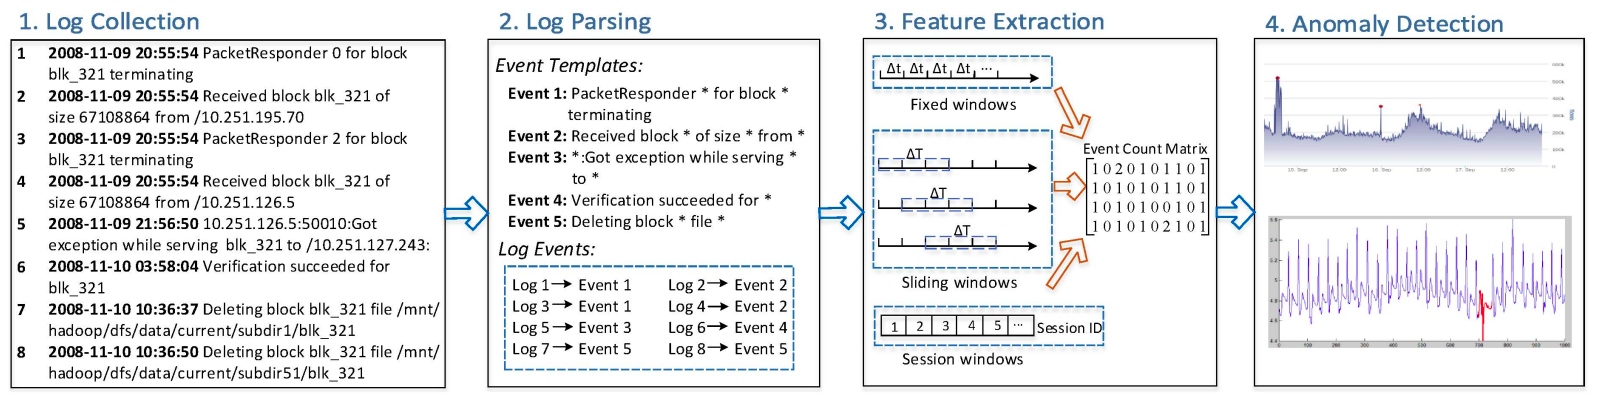
\includegraphics[width=\linewidth]{figures/anomaly-detection.png}
    \caption{Framework of anomaly detection. Retrieved from~\cite{he2016expreport}.}
    \label{fig:anomaly-detection}
\end{figure}

\subsection{Log collection}
Large-scale systems generate logs as a standard practice to record system states and runtime information. Each log entry typically consists of a timestamp and a message indicating the event or action that occurred.~\cite{he2016expreport}

\subsection{Log parsing}
Log parsing aims to structure unstructured logs by extracting event templates from free-form text. Each log message is parsed into an event template consisting of a constant part and specific parameters.~\cite{he2016expreport}

There are two types of parsing methods~\cite{he2016expreport}:
\begin{enumerate}
    \item Clustering-based method \--- Computing distances between logs and then use clustering techniques to group them into clusters. The event templates are then generated from each cluster.
    \item Heuristic-based method \--- Counting the occurrences of each word at each log position. Then, frequent words are selected and combined as event candidates, from which some are chosen to be the log events.
\end{enumerate}

\subsection{Feature extraction}
The next step is to encode logs into numerical feature vectors for machine learning models. This process involves slicing the raw logs into log sequences using various grouping techniques~\cite{he2016expreport}:

\begin{enumerate}
    \item Fixed window \--- This approach relies on a timestamp that logs the time of each occurrence. Every fixed window has its own size, indicative of the time span or duration. The size of the window is represented by a constant value \--- $\Delta t$.
    \item Sliding window \--- Consists of two attributes: the size of the window and the size of the step. The step size is less than the window size, which results in the overlapping of various windows.
    \item Session window \--- This method is based on identifiers rather than timestamps. These identifiers serve to distinguish various execution routes in certain log data.
\end{enumerate}

Once we have generated log sequences using windowing, it allows us to construct an event count matrix X. Within each log sequence, we count the frequency of each log event to create the event count vector. To illustrate, [0, 0, 2, 3, 0, 1, 0] means that event 3 took place twice, and event 4 occurred three times.~\cite{he2016expreport}

\subsection{Anomaly detection}
Once the feature matrix is prepared, it can be inserted into machine learning models for training. These models are then used to generate a model specifically designed for anomaly detection.~\cite{he2016expreport}




\chapter{Modeling log events}
\label{chap:modeling}


\chapter{Implementation}
\label{chap:implementation}


\chapter{Experiments}
\label{chap:experiments}


\chapter{Testing}
\label{chap:testing}


\chapter{Conclusion}
\label{chap:conclusion}
